\documentclass[logo,reportComp]{thesis}
\usepackage[python,pseudo,linenum]{mypackage}
\usepackage{relsize}

\setcounter{secnumdepth}{4}
\titleformat{\paragraph}{\bfseries}{\alph{paragraph})~~}{0em}{}
\titlespacing*{\paragraph}{0pt}{0pt}{0pt}[0pt]

\title{多核程序设计}
\subtitle{作业一:计算二维数组中心熵}
\school{数据科学与计算机学院}
\author{陈鸿峥}
\classname{17大数据与人工智能}
\stunum{17341015}
\headercontext{多核程序设计作业}

\let\emph\relax % there's no \RedeclareTextFontCommand
\DeclareTextFontCommand{\emph}{\kaiti\em}
\AtBeginEnvironment{quote}{\kaiti\small}

\begin{document}

\maketitle
\tableofcontents

\newpage

\section{题目描述}
计算二维数组中以每个元素为中心的熵(entropy)
\begin{itemize}
    \item 输入:二维数组及其大小,假设元素为$[0,15]$的整型
    \item 输出:浮点型二维数组(保留$5$位小数)
    \begin{itemize}
        \item 每个元素中的值为以该元素为中心的大小为$5$的窗口中值的熵
        \item 当元素位于数组的边界窗口越界时,只考虑数组内的值
    \end{itemize}
\end{itemize}
\begin{figure}[H]
\centering
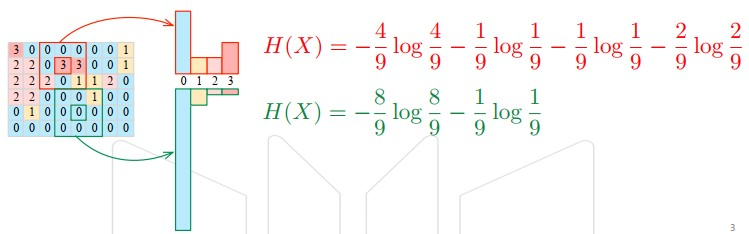
\includegraphics[width=0.9\linewidth]{fig/entropy.jpg}
\end{figure}

回答以下问题:
\begin{enumerate}
\item 介绍程序整体逻辑,包含的函数,每个函数完成的内容。(10分)
\begin{itemize}
    \item 对于核函数,应该说明每个线程块及每个线程所分配的任务
\end{itemize}
\item 解释程序中涉及哪些类型的存储器(如,全局内存,共享内存等),并通过分析数据的访存模式及该存储器的特性说明为何使用该种存储器。(15分)
\item 程序中的对数运算实际只涉及对整数$[1,25]$的对数运算,为什么?如使用查表对$\log1\thicksim \log25$进行查表,是否能加速运算过程?请通过实验收集运行时间,并验证说明。(15分)
\item 请给出一个基础版本(baseline)及至少一个优化版本,并分析说明每种优化对性能的影响。(40分)
\begin{itemize}
    \item 例如,使用共享内存及不使用共享内存
    \item 优化失败的版本也可以进行比较
\end{itemize}
\item 对实验结果进行分析,从中归纳总结影响CUDA程序性能的因素。(20分)
\item 可选做:使用OpenMP实现并与CUDA版本进行对比。(20分)
\end{enumerate}

\section{原理推导}
设窗口大小为$M\times M$,本题中$M=5$,由题意知中心熵为窗口内合法元素的熵之和。
设窗口内合法的元素数目为$N$,每个元素值的数目为$N_i(i=0,\ldots,15)$,则有中心熵的计算公式
\begin{equation}
\label{equ:ent}
H(X)=\sum_{i=0}^{15}-\frac{N_i}{N}\log\frac{N_i}{N}\;,
\end{equation}
且满足$N=\sum_{i=0}^{15} N_i$。

对式(\ref{equ:ent})进行变换有
\begin{align}
H(X) &= -\frac{1}{N}\sum_{i=0}^{15}N_i(\log N_i-\log N)\\
&= -\frac{1}{N}\sum_{i=0}^{15}N_i\log N_i + \log N
\end{align}
进而可降低除法的次数,缩短计算时间。

同时可以看到这里的运算变成了整数的对数运算,由于$N_{\max}=M\times M=25$,因此可以先计算出$[1,25]$的所有对数值,然后通过查表法实现上述运算。

\section{程序逻辑}
在本次实验中我实现了五个版本的程序,包括基础的NumPy实现、OpenMP实现以及CUDA三个版本的实现。

这里几个版本分别对应着CPU的单核程序、CPU的并行程序以及GPU的并行程序。

\subsection{NumPy实现}
之所以选择NumPy将本次实验进行实现,一方面是为了提供Baseline程序用于结果验证,另一方面则是尝试探索利用CPU计算性能可以达到多高。
NumPy虽然是Python的库,但是其底层代码都是采用C进行编程,并且利用了Intel的MKL库,因此性能其实是很高的,作为CPU Baseline也相当合适。

在Python里实现起来也相当方便,对于数组内的每一元素遍历,通过NumPy数组的切片(slicing)访问,可以得到每个中心点对应的窗口,并对其计算直方图,最终利用向量计算即可求得中心熵。
核心代码如下所示。
\lstinputlisting[firstline=26,lastline=49]{../numpy/main.py}

NumPy实现的亮点在于高效的\textbf{向量化操作},而非普通的裸串行代码。
完整代码请见\verb'numpy/main.py'。

\subsection{OpenMP实现}
接下来我采用C++实现了CPU的并行版本,利用OpenMP进行加速,测试并行后的性能。

C++的代码逻辑没有Python那么紧凑,但是还是非常清晰的。
外层两层循环遍历输入数组中的每一个元素,内层两层循环计算直方图。

注意到这里为了跟CUDA的实现保持一致,输入统一采用一维数组存取,需要先计算出下标\verb'idx'再去读取数据。
详细步骤如下:
\begin{enumerate}
\item 对于矩阵中的每个点,统计其周围$5\times 5$窗口内每个元素出现的次数。
这里直接开设大小为$16$的桶\verb'cnt',每次遇到一个元素就往对应桶里加$1$。
由于窗口超出原矩阵范围的点不纳入计算,因此需要另外采用变量\verb'valid'记录合法元素数目。
\item 等遍历完该点对应窗口中的所有元素,按照熵的公式进行累积。
\item 采用公式\ref{equ:ent}对累积和进行操作,得到最终的中心熵。
\end{enumerate}

为利用多核的并行计算能力,直接在最外层循环添加\verb'#pragma omp parallel for'。
由于内层循环并没有发生共享内存的写冲突,因此无需采用原子操作等来对线程进行同步。
核心代码逻辑如下,完整代码可见\verb'openmp/src/core.cpp'。

\lstinputlisting[firstline=13,lastline=60,language=c++]{../openmp/src/core.cpp}

这里需要注意,由于C++没有Python中的切片功能,因此需要人工判断数组是否越界。
同时,OpenMP的实现中也给出了两种不同计算$\log$值的方式,一种采用预设好的对数表进行查表计算(开启\verb'LOOKUP'的宏),另一种则采用\verb'<math.h>'库中的\verb'log'函数。
两种方法的比较会在最后的实验部分(第\ref{sec:exp}节)给出。

\subsection{CUDA实现}
然后我又着重在GPU上实现并优化了本次作业的内容。

\subsubsection{基线版本}
基线版本的CUDA程序与OpenMP的实现非常相似,不同之处在于CUDA的实现需要用\verb'__global__'来声明核函数,同时在核函数内部只用考虑单一线程的计算情况,因此只需描述内部窗口的两层循环。

其他计算过程与OpenMP一致,即统计直方图,并计算中心熵。
这里同样提供了使用查找表和不使用查找表算对数的方法,后文实验中会做详细比较。

核函数如下所示,完整代码请见\verb'sources'文件夹。
\lstinputlisting[firstline=16,lastline=61,language=c++]{../sources/src/core.cu}

基础版本采用一维的Grid和一维的Block,因为本来输入也是线性的,故在计算坐标时稍微转换一下即可。
每个Block内开$1024$个线程,共开$\lceil W\cdot H/1024\rceil$个Grid,这里的$W$和$H$分别为输入矩阵的宽和高。
每个线程都计算某一点的中心熵。
\lstinputlisting[firstline=81,lastline=82,language=c++]{../sources/src/core.cu}

\subsubsection{二维线程块版本}
第二个版本的CUDA程序采用了二维的Grid和Block,通过对原输入矩阵进行tiling操作,即可将原矩阵划分成多个小矩阵。
每个Block计算一个小矩阵,而Block内的每一个线程则对小矩阵内的对应元素计算中心熵。

这里利用\verb'dim3'创建二维的Grid和Block,并按照如下方式调用核函数。
\lstinputlisting[firstline=87,lastline=90,language=c++]{../sources-2d/src/core.cu}

核心代码逻辑依然跟上述的基线版本相同,变化的只是下面的坐标映射部分。
完整代码可见\verb'sources-2d'文件夹。
\lstinputlisting[firstline=30,lastline=32,language=c++]{../sources-2d/src/core.cu}

\subsubsection{共享内存版本}
注意到程序中涉及到大量输入矩阵的读取,计算每个点的中心熵都需要将周围$5\times 5$的所有元素读入,这显然是一个很大的开销。
前面两个版本的程序都是将输入矩阵放在全局内存中,那么可以考虑将部分元素提前读入共享内存,以实现加速的读取。

依然采用二维线程块划分的思路,如果对于每个块,将其对应的所有元素迁移到共享内存,那似乎就可以达成上述目的。
但事实上在计算该块每个元素的中心熵时,往往还需要周围一些块的对应的元素,因此如果仅仅将块内的元素读入到共享内存则会发生访问错误的问题,因为边界元素未被读入。
故正确的方式应该是将块内及块周围的元素都一并读入,然后再做计算。

这里我采用了padding的方法,比如对于一个$16\times 16$的Block,那么开$(16+2\times 2)^2=20^2=400$个线程,对这个Block周围一圈宽度为$2$的部分也一并读入共享内存。
对于这些线程来说,每个线程只要读取它对应的那个元素到共享内存即可,并在读取完成后利用\verb'__syncthreads'同步线程。
需要考虑两个边界情况:
\begin{itemize}
	\item 如果线程对应的元素超出原始矩阵的范围,那么直接置$0$(不做读入)。
	\item 如果线程对应的元素在原始矩阵的范围内,但超出了该块对应的范围,那么依然需要算出原始矩阵元素的坐标,并读入共享内存。
\end{itemize}
代码逻辑如下:
\lstinputlisting[firstline=31,lastline=43,language=c++]{../sources-shared_mem/src/core.cu}

下面的中心熵计算逻辑基本与前面的方法一样,只是读取数据直接从共享内存中读取即可。
另外需要判断当前线程是否是在合法的块内(而不是padding的部分),如果是padding的读入线程,那么其在计算环节将会被闲置(主要是任务不好划分,如果将其也加入到计算中,很容易引起负载不均的问题)。
由于padding读入的线程数和实际计算的线程数不同,线程对应的ID映射也需要非常小心。
如下,Grid的划分数目对应原始块的大小,但Block里的线程数目则是要通过padding后的块大小决定。
\lstinputlisting[firstline=102,lastline=104,language=c++]{../sources-shared_mem/src/core.cu}

这里只放出与前面的版本相比有改动的部分,完整代码请见\verb'sources-shared_mem'文件夹。
\lstinputlisting[firstline=44,lastline=59,language=c++]{../sources-shared_mem/src/core.cu}

\section{实验结果}
\label{sec:exp}

\section{实验心得}

% \begin{thebibliography}{99}
% https://www.evl.uic.edu/sjames/cs525/final.html
% https://tvm.apache.org/docs/tutorials/optimize/opt_conv_cuda.html
% \end{thebibliography}

\end{document}

% 评分细则
% – 程序正确性 40
% – 编程规范 10
% • 初始分 10
% • 缺少文件头 -5
% • 缺少函数头 -5
% • 换行没有正确缩进 -5
% • 函数过长 -5
% – 书面报告 100

% 提交作业
% – 邮箱:
% multicoresysu2020@163.com
% – 截止时间
% • 7月5日晚23:59
% • 如需使用slip days,请于截止时间前将需要使用的天数发送至提交作业邮箱

% 提交文件结构说明
% – your name-your ID
% • README (实验报告)
% • sources
% – all sources files
% – Makefile